\documentclass[12pt,oneside]{report}

%%% Load some useful packages:
%% "New" LaTeX2e graphics support.
\usepackage{graphicx}
%%	using final option to force graphics to be included even in draft mode
%\usepackage[final]{graphicx}
%% Tell graphicx the default directory for all figures
\graphicspath{{figures/}}

%% Enable subfigure support
\usepackage{subfigure}

%% Make subsubsections numbered and included in ToC
\setcounter{secnumdepth}{3}
\setcounter{tocdepth}{2}

%% Package to linebreak URLs in a sane manner.
\usepackage{url}

%% Define a new 'smallurl' style for the package that will use a smaller font.
\makeatletter
\def\url@smallurlstyle{%
  \@ifundefined{selectfont}{\def\UrlFont{\sf}}{\def\UrlFont{\small\ttfamily}}}
\makeatother
%% Now actually use the newly defined style.
\urlstyle{smallurl}

%% Define 'tinyurl' style for even smaller URLs (such as in tables)
\makeatletter
\def\url@tinyurlstyle{%
  \@ifundefined{selectfont}{\def\UrlFont{\sf}}{\def\UrlFont{\scriptsize\ttfamily}}}
\makeatother

%% Provides additional functionality for tabular environments
\usepackage{array}

%% Puts space after macros, unless followed by punctuation
\usepackage{xspace}

%% Make margins less ridiculous
\usepackage{fullpage}

%% Allows insertion of fixme notes for future work
\usepackage[footnote, nomargin]{fixme}

%%%% Turned off for tech report, should be turned on for research portfolio
%% Turn on double spacing
\usepackage{setspace}
\doublespacing

%% Make URLs clickable
%\usepackage[colorlinks, bookmarks=false]{hyperref}
\usepackage[colorlinks, bookmarks=true]{hyperref}

%% Since I'm using the LaTeX Makefile that uses dvips, I need this
%% package to make URLs break nicely
\usepackage{breakurl}

\usepackage{amsmath,amsfonts}
\numberwithin{equation}{subsection}
%%\usepackage{nonfloat}
\usepackage{bbm}
\usepackage{setspace}
\onehalfspacing
\usepackage{tabularx}

%%% End of preamble
\begin{document}

\title{Dissertation proposal: \\ [1.0cm]
       \textsc{Software Trajectory Analysis:} \\
       \textsc{An empirically based method for automated software process discovery} \\
       \author{Pavel Senin \\
							 Collaborative Software Development Laboratory \\
               Department of Information and Computer Sciences \\
               University of Hawaii \\
               \texttt{senin@hawaii.edu} \\ [0.6cm]
               CSDL Technical Report 09-09 \\
               \url{http://csdl.ics.hawaii.edu/techreports/09-09/09-09.pdf}
       }
       \date{August 2009}
}
\maketitle

\clearpage

%% Philip suggests it needs a ToC
\tableofcontents

%\begin{abstract}
%Abstract goes here if needed.
%\end{abstract}

%% Start with introduction
\chapter{Introduction}\label{chapter_introduction}
\textit{The central issue I address in the dissertation is a possibility of recurrent behaviors discovery from 
publicly available software process artifacts by leveraging data mining and knowledge discovery techniques. 
In particular I explored an approach of discovering of recurrent behaviors through the mining of time series that
are constructed by temporal ordering of measurements extracted from software process artifacts.
Further, I shall propose a novel technique for characteristic patterns discovery from time series and show its 
applicability to the problem at hands.}

\textit{The problem's background is provided in the Section \ref{section_background}. 
Section \ref{section_software_process_design} presents classical approaches for software process design and shows its limitations.
Section \ref{section_research_hypothesis} introduces the research hypothesis.
Section \ref{knowledge_discovery} provides a background into the problem of knowledge discovery 
from time-series.
Section \ref{section_trajectory_definition} connects two problems and provides definitions.
Section \ref{section_contributions} enumerates main contributions of the thesis, 
while section \ref{section_organization} explains the thesis organization.}

%
% >> section
%
\section{Background}\label{section_background}
Contemporary software projects concern with development of complex software systems and typically have 
a considerably long life-cycle - well over decade.
A project's development and maintenance activities are usually carried out by geographically 
distributed teams and individuals. The development pace, the experience, and the structure of the 
development team continuously change with project progression and as developers joining and leaving. 
When combined with schedule and requirements adjustments, these create numerous difficulties 
for developers, users, and stakeholders, ultimately affecting the project success \cite{citeulike:2207657}. 

This software development complexity phenomena was identified in 1968 as ``Software crisis'' 
\cite{naur_crisis_68}, and was addressed by bringing the research and the practice of software development 
(or as it was called ``programming'') under the umbrella of Engineering - in an effort to provide 
the control over the process of software development. 
Following the engineering paradigm, numerous methodologies and models of software design and development 
process, known as \textit{software processes}, were proposed \cite{citeulike:10002165}.

\begin{defn}\label{def_process}
A \textbf{\textit{Software Process}} defines a sequence of activities performed in order 
to design, develop, and maintain software systems.
\end{defn}
Examples of such activities include requirements collection and creation of UML diagrams, 
requirements testing, code development,  testing, etc. The intent behind a software process is 
to provide a control over software evolution by implementing a global strategy and by structuring
and coordinating human activities in order to achieve the goal - deliver a functional software system 
on time and under the budget. 

Since then, much research has been done on software processes resulting in a number
of software development models and paradigms. Some of these were widely accepted by practitioners 
and evolved into industrial standards for software development processes such as CMM, ISO, PSP, 
and others \cite{citeulike:5043104}. However, in spite of this effort, industrial software 
development remains error-prone and more than half of all 
commercial software development projects ending up failing or being very poorly executed 
(Rubinstein, ``Chaos Reports'', 2006) \cite{chaos2006}. Some of them are abandoned due to running 
over budget, some are delivered with such low quality, or so late, that they are useless, and some, 
when delivered, are never used because they do not fulfill requirements. 

Through the analyses of software project failures, it was acknowledged, that the engineering 
paradigm might not be the best way to provide a control over software development processes 
(\cite{citeulike:3729379} \cite{citeulike:5203446}) due to the fact that Software engineering 
is dealing with significantly different from other Engineering fields problems \cite{citeulike:2207657} .
The chief argument supporting this point of view is the drastic difference in the cost model:
while in Software Engineering there is almost no cost associated with materials and 
fabrication, these usually dominate cost in all other Engineering disciplines, but, 
ironically, Software Engineering is suffering from the costs and challenges associated with 
continuous re-design of the product and its design processes - the issue which is 
hardly seen at all in other Engineering areas. 
Further, it was found, that most of the engineering-like models are rigid, ``context-free'',
and rather prescriptive, i.e. they are universally defined independently of a particular 
organizational structure or a project specificities \cite{sacchi_2001}, and while they 
structure processes and provide the control, following them does not guarantee the success.
Yet another argument supporting alternative to engineering approaches is the increasing 
understanding and appreciation of a human role in software development processes over tools, 
technologies, and standards \cite{citeulike:6580825} \cite{citeulike:149387}
\cite{1605185} \cite{citeulike:113403} \cite{1605188} \cite{citeulike:12743107}. 

Along with Software Engineering, a number of alternative, flexible and user-oriented software processes 
emerged from academy, hobbyists, and practitioners addressing aforementioned issues \cite{citeulike:3729379}. 
Among others, the Free/Libre/Open-Source Software model (FLOSS) and the software craftsmanship  
approaches gained a significant credibility in community. 
While the former \textit{holistic} software process paradigm emphasizes loosely-organized 
collaboration, frequent releases, and effectively removes the boundary between developers 
and customers, the latter, human-centric approach, is built upon the roles of highly 
motivated skilled individuals \cite{citeulike:262020} \cite{citeulike:2759198}. 

Nevertheless, alternative processes were found to be plagued by the same complexity issues. 
As it was shown, most of FLOSS projects never reach a ``magic'' 1.0 version \cite{citeulike:12480029}. 
Among others, the great "infant mortality rate" of FLOSS projects was related to a burnout, 
inability to acquire a critical mass of users, loss of leading developer(s), and forking \cite{richter2007critique}. 
Software craftsmanship, from other hands, not only challenges developers with technological advances 
requiring continuous skills improvement, but creates significant cost and effort estimation difficulties for
stakeholders and project managers \cite{citeulike:11058784}. However, despite to these issues, 
the alternative processes proved that the disciplined manner of programming and the modularization  
of the software are capable of delivering large and reliable software systems, most notable Linux OS,
suggesting that community-driven processes as good as industrial engineering-like processes.

Currently, it is widely acknowledged, that there exists no single ``silver bullet'' process which 
can bring a software development project to success \cite{citeulike:1986013}. 
Processes are numerous, each has advantages and drawbacks, and each is accompanied with 
numerous application recommendations, success stories, and with failure experiences. Nevertheless,
the alarming rate of failing projects suggests that our understanding of software process ``mechanics''  
is limited and insufficient\cite{citeulike:12550665}. 
The enormous cost of the lost effort, measured in hundreds of billions of US dollars 
\cite{citeulike:2207657} \cite{citeulike:2207653} \cite{citeulike:2207655}, 
continues to provide motivation for further research on software processes. 

%
% >> section
%
\section{Software process design}\label{section_software_process_design}
Traditionally, approaches to software process design and improvement are divided into two distinct categories. 

The first category of software process design approaches consists of traditional to engineering 
\textit{top-down} prescriptive techniques through 
\textit{proposing a process based on specific patterns of software development}. 
For example, the Waterfall Model process proposes a sequential pattern in which developers first create a 
Requirements document, then create a Design, then create an Implementation, and finally develop Tests. 
The Test Driven Development process, from other hands, proposes an iterative behavioral pattern in which
the developer must first write a test case, then write the code to implement that test case, then re-factor the 
system for maximum clarity and minimal code duplication \cite{citeulike:6086365}. 

While the top-down approach follows the usual path of trials and errors, and seems to be an extension 
of natural to humans creative processes of invention and experimentation, 
the ``invention'' of an adequate to the task software process is far from trivial 
\cite{citeulike:5043104} \cite{citeulike:1986013}. Moreover, an evaluation cycle of an invented process
is usually very expensive and considerably long.
In addition, it was shown that the process inventors are often limited in their scope and tend to assume 
idealized versions of real processes, thus, often produce ``paper lions'' - process models which are 
likely to be disruptive and unacceptable for end users, at least in their proposed form 
\cite{citeulike:9758924}, which creates a large discrepancy between actions that supposed to be done for 
the novel process and what was actually performed by particular individual or the team.

The second category of software design approaches consists of \textit{bottom-up} techniques 
that focus on a \textit{performed process reconstruction through noticing of recurrent development 
events and behaviors} or as it also called \textit{process enactment}. 
Usually, the process reconstruction task is viewed as a two-levels problem where the first level 
consists of a patterns discovery (segmentation) while the second level consists of patterns recognition 
and their network analysis \cite{citeulike:2703162}.
One of the first works in this category was by Cook and Wolf, where they show a
possibility of automated extraction of a process model through the mining of recorded 
process event logs \cite{citeulike:328044} \cite{citeulike:5120757} \cite{citeulike:5128143}. 
Later work by Huo et al. shows that it is also possible to improve an existing process
through the event logs analysis \cite{citeulike:7691059} \cite{citeulike:7690766}. 

While the bottom-up approaches seem to be more systematic and potentially less complex than invention, 
they also affected by a number of issues. A chief among these is the observability issue - 
it is usually very difficult to conduct a full depth study on a live project due to the privacy concerns. 
Moreover, it is expensive to observe a process performed by a team for a whole life-cycle of a project. 
Yet another issue is the capacity of currently available process discovery techniques - 
typically these need to be supervised by experts and finely tuned in order to reconstruct 
distributed and concurrent processes. 

Nevertheless, despite to their differences, both techniques for software process design are 
producing process models that effectively are the series of actions that must be performed successively 
(sequentially and sometimes iteratively) in order to deliver a software. 
In order to produce the viable model, the ``process inventors'' put the best of their knowledge, experience,
creativity, and logical reasoning into the proposed sequence of steps, while ``process re-constructors 
strive to eliminate the noise and to converge to a concise process model that is supported by the 
majority of observations. 
This attention to synthesis of sequential steps, leaves other phenomenas, such as team's structure, work schedule, 
developer's discipline, their behaviors, and motivation behind. While this issue was recognized previously
and resulted in a number of studies which called for attention of human element in software production 
\cite{citeulike:149387} \cite{citeulike:113403} \cite{citeulike:205322} \cite{citeulike:12798652}, 
it is still largely ignored in industrial practices \cite{citeulike:12798659}, mostly due to the 
difficulties in benefit estimation \cite{citeulike:12798662} \cite{csdl2-12-11}.

%
% >> section
%
\section{Free/Libre Open Source processes}\label{floss_processes}
Along with growing amount of publicly available software, it became obvious, that self-organizing communities of 
mostly ``recreational'' software developers and active users are capable to successfully manage large code base, 
but to deliver software increasingly complex and surprisingly popular.
Many of large, ``global'' open source software development projects, such as Linux and its derivatives, 
Gnome, Apache HTTP Server, MySQL, and others, not only have comparable with industrial projects development team 
and code-base sizes, but the same average defect rate \cite{coverity2012}. 
These facts have attracted a considerable attention from industry and many organizations 
seek to emulate successful open source software processes in traditional ``closed source'' environment 
\cite{oss_virtual_organizations} \cite{oss_balance} \cite{oss_hp} \cite{oss_4industry}. 

\begin{figure}[ht!]
   \centering
   \includegraphics[width=140mm]{figures/Linus.Kernel.ps}
   \caption{A Torvald's response suggesting that practical reasons, the ``real-life'', should be always considered 
   over specifications.
   Excerpt from the Linux mailing list. \url{http://lkml.indiana.edu/hypermail/linux/kernel/0509.3/1441.html}}
   \label{fig:kernel}
\end{figure}

If we consider this as an assertion that open-source software processes are at least as good as engineering-like 
software process models, then, the freely available open-source process software artifacts potentially bear an 
incredible wealth of the information worth of studying. Moreover, the striking differences of open-source processes 
from a traditional software development could potentially reveal novel software processes and their aspects that 
were previously not accounted for. 
For example, consider that the most significant document in industrial software processes - a specification - 
is rarely considered at all in open source world. In FLOSS projects the software look and its functionality are 
rather viewed as open-end questions. Even in the Linux kernel development, which is probably one of the few strictly 
moderated FLOSS development processes, developers prise practical reasons over specifications 
\ref{fig:kernel}.

Yet another source of motivation for studying of public FLOSS software process artifacts comes from the fact that 
in order to facilitate the distributed FLOSS software development processes, the community is highly encouraging
developers to commit their changes rather often \cite{so-checkin} \cite{git-best-practices1}.
The frequent commits and the changes visibility practice is often cited as vital for health of software 
process as mentioned in some lengthy discussions: ``\textit{Don't Go Dark}'' \cite{checkin-dgd-2008}, 
``\textit{Check In Early, Check In Often}'' \cite{checkin-ch-2012}. Potentially, frequent commits create artifacts 
trails that provide finer resolution into project development and allow more thorough process recovery.

%
% >> section
%
\section{Public software repositories}\label{section_public_repositories}
Recently, the aforementioned situation changed, and the interest for process enactment and reconstruction, 
as well as attention to the human-specific components of software processes has been revived. 
This change is driven by the increase in public data that are made available by the proliferation of open 
source communities.

Currently, with accessible personal computers, friendly software development toolkits, and due to massification
of the use of the web as
a platform for collaborative work, small-scale commercial and recreational 
programming become very popular. 
Today, free code hosting sites such as SourceForge, GoggleCode, and GitHub host thousands of 
Free/Libre Open Source Software (FLOSS) projects.
These publicly offer numerous software artifacts such as design documents, source codes, bugs and issue records, and 
developers and users communications.
Further, Q\&A and social websites for developers such as StackOverflow, Biostars, TopCoder and others becoming 
increasingly popular among the software developers as places for exchanging experiences, learning new tricks, and 
improving skills, plus, they offer anonymized data back to the community.

The public availability of numerous software process artifacts effectively removes not only the high cost of observation, 
but most of the privacy concerns - the two issues that previously made any large-scale analysis of software projects 
unfeasible for most researchers.

Scientific community response on the availability of public artifacts was overwhelming, and a number of 
venues was established addressing the increased interest. 
Since 2004, the International Conference on Software Engineering (ICSE) hosts a Working Conference on 
Mining Software Repositories (MSR). The original call for papers stated MSR's purpose as 
\textit{``... to use the data stored in these software repositories to further understanding of software 
development practices ... [and enable repositories to be] used by researchers to gain empirically based 
understanding of software development, and by software practitioners to predict and plan various aspects 
of their project''} \cite{msr2004} \cite{citeulike:7853299}. 
Several other venues: International Conference on Predictive Models in Software Engineering \cite{promise12}, 
International Conference on Open Source Systems, the Workshop on Public Data about Software Development, 
and the International Workshop on Emerging Trends in FLOSS Research have also played
an important role in shaping and advancing this research domain.

Some of the published work addresses the software process discovery. Among others, most notable and 
relevant to my research is work by Jensen \& Scacchi. In their early work, they demonstrated, that 
information reflecting software processes can be gathered from public systems \cite{citeulike:12550640}. 
Later, in \cite{citeulike:5043664} and \cite{citeulike:5128808}, they show, that by manual mapping of 
collected process evidence to a pre-defined process meta-model it is possible to reconstruct some 
of the FLOSS processes. 
Another closely related to my research is work by Hindle et al. where they has shown that it is possible to 
discover software process evidence through partitioning \cite{citeulike:10377366}.

However, the research work based on mining of software process artifacts shows, that while public availability 
of artifacts is minimizing observability and privacy issues, the nature of these artifacts creates a number of 
challenges which I discuss in the chapter X, which limit the possible scope of the research and significantly 
elevate the complexity of the process discovery effectively rendering previously designed techniques inefficient.
Thus, the novel analysis and discovery techniques are needed to be developed for public software process artifacts 
analysis \cite{citeulike:7853299}.
% when ``\textit{... going beyond code and bugs...}'' 

%
% >> section
%
\section{Research hypothesis, scope of the dissertation}\label{section_research_hypothesis}
In previous sections, I have outlined the evidence of a limited performance of existing engineering-like 
software processes (Section \ref{section_background}),
as well the oversight of a variety of human factors that fall beyond a typical sequence of development 
actions by traditional approaches to software process design (Section \ref{section_software_process_design}).
Then, I have identified a few differences of FLOSS processes from traditional Software Engineering 
(Section \ref{floss_processes}), which can potentially shed light on human-driven aspects of software development.
Finally, I have pointed out a growing wealth of publicly available software process artifacts 
(Section \ref{section_public_repositories}) that is worth to explore for a better understanding not only 
FLOSS software processes, but their human factors. All this provided a motivation to my exploratory study, 
whose details I outline in this section.

In my work, I attempted to explore the possibility of discovery of a specific human-driven aspect in 
FLOSS software development that is a \textit{\textbf{behavior}}, which I define as the mannerism in which a 
developer, or a team, conduct their everyday work. 
In particular, I explore the possibility of discovery of \textit{recurrent behaviors}, i.e. behaviors supported 
by a numerous evidence, from software process artifacts. 

For example, if within an observation interval one developer frequently runs unit tests before committing 
changes into repository, while another usually commit changes without running the tests, the first developer's
habit of testing a code before the commit is a recurrent behavior that may reflect the developer's discipline,
or an unusual attention to some particular part of the code. 
Consider another example, if one of the developers usually commits code changes in mornings, while another 
developer late in the day, these two recurrent behaviors, might indicate a constraints that are put on the 
project, or the process, or on the developers themselves.
Obviously, latter behaviors should be possible to quantify by simple analysis of commit timestamps, while 
the former can be discovered by the analysis of co-occurring changes in the source code. 
Moreover, these and similar recurrent behaviors could be further associated with certain project's or process 
traits, such as pace, agility, size, complexity, code quality and others, which will not only extend our 
knowledge of human factors in software processes, but will lay a foundation for future research in software 
processes.

To begin with, I hypothesized, that \textbf{\textit{it is possible to discover recurrent behaviors from 
publicly available software process artifacts}}. 

Following the hypothesis, I have investigated a number of publicly available software repositories,
their artifacts, and a number of applicable data-mining techniques in a preliminary exploratory study 
\cite{csdl2-10-09}. However, similarly to other studies in the field, I have discovered, that while FLOSS 
process artifacts are numerous and readily accessible, their irregular, snapshot-like nature and the poor 
informational content significantly limit the applicability of known techniques for process mining.

In order to overcome this issue, I have casted the initial problem of event-based recurrent behaviors 
discovery into more generic problem of knowledge discovery from time series and approached it
by developing a novel technique for interpretable comparative analysis of time series that allows 
characteristic patterns discovery and ranking called SAX-VSM \cite{sax-vsm}. 

Further, I have developed a software artifacts analysis framework, called Software Trajectory Analysis, 
which aids in software artifacts collection, software process and product evolutionary metrics extraction, 
and their comparative analyses that enable discovery and ranking of characteristic patterns.


 in rank highlight is  transformation into  and by using I approached the problem of knowledge discovery 

developed a 
software process artifacts mining framework called Software Trajectory Analysis which is built upon 
a novel technique for comparative analysis of time series that allows characteristic patterns discovery 
and ranking.

This dissertation presents its results, as well as introduces a novel data mining technique designed to 
alleviate difficulties with interpretability of quantitative results obtained through mining of software
artifacts trails. 

%
% >> section
%
\section{Knowledge discovery from time series}\label{section_knowledge_discovery}
In data mining, time series are used as a proxy representing a vast variety of real-life phenomena 
in wide range of fields including, but not limited to physics, medicine, meteorology, 
music, motion capture, image recognition, signal processing, and text mining. 
While time series usually directly represent observed phenomenas by capturing their measurable evolution in time, 
the pseudo time series often used for representation of various high-dimensional data 
by combining data points into ordered sequences. 
For example in spectrography data values are ordered by component wavelengths \cite{citeulike:12550833};
in shape analysis the order is the clockwise walk direction starting from a
specific point in the outline \cite{citeulike:12550835}, in image classification the numbers of pixels
are sorted by color component values \cite{citeulike:2900542}.

Many important problems of knowledge discovery from time series reduce to the core task of finding 
characteristic, likely to be repeated, sub-sequences in a longer time series. 
In the early work these were called as 
\textit{frequent patterns} \cite{citeulike:5159615}, 
\textit{approximate periodic patterns} \cite{citeulike:1959582},
\textit{primitive shapes} \cite{citeulike:5898869}, 
\textit{class prototypes} \cite{citeulike:4406444}, 
or \textit{understandable patterns} \cite{citeulike:3978076}. 
Later, similarly to Bioinformatics, these were unified under the term \textit{motif} \cite{citeulike:3977965}.
Once found, motifs can be used for a hypothesis generation by finding their associations with known,
or unknown phenomenas \cite{citeulike:3977965}. 

The recent advances in semi-supervised and unsupervised finding of such characteristic sub-sequences, 
in particular work based on \textit{shapelets} \cite{citeulike:7344347} \cite{citeulike:11957982}
\cite{citeulike:12552293} and \textit{bag of patterns} \cite{citeulike:10525778}, show a great potential 
of application of time series data-mining techniques to a wide variety of high-dimensional data.

Unfortunately, both techniques provide a limited insight into the data and suffer from performance issues. 
While exact shapelet techniques allow discovery of class-characteristic patterns and facilitate classification,
algorithm is almost quadratic and provides limited insight into class specificities. 
The bag of patterns algorithm, while performs in a linear time, requires a previous knowledge for input parameters 
selection and does not offer class generalization.

In order to overcome this limitations, in this thesis I propose a novel approach for time-series classification and 
knowledge discovery that is called SAX-VSM and is based on symbolic approximation of time series and vector space model. 
As I shall show, SAX-VSM is capable to discover and to rank characteristic subsequences representing time series classes. 
The proposed algorithm not only facilitates classification, but provides insights into the both: classification results 
and time series classes specificities. As I shall show, by facilitating the class' characteristics patterns ranking,
SAX-VSM enables the discovery of recurrent behaviors and their heat-map like visualization. 

\section{Software trajectory analysis}\label{section_trajectory_definition}
Previously, Johnson et al. defined \textit{software metrics telemetry streams} \cite{citeulike:12550871}, 
(what they re?) and showed, that it is possible to improve software development process by using the 
knowledge extracted by experts through visual analysis of these streams.
 
Similarly to software metrics telemetry streams, I abstract software process artifact by collecting their 
metrics and arrange these measurements by artifact creation time into high-dimensional vectors. 
These non-equidistant, often sparse and uneven in length time series 
I call ``\textbf{software trajectories}''. Similarly to approximate trajectories of objects in 
a physical space, or reduced in complexity sequence of states of a dynamic system (Poincare' maps), 
the \textit{software trajectory is a curve that describes a software project progression in a space 
of a chosen metrics}.

Through an exploratory study, I have discovered, that by the comparative analysis of software trajectories 
with SAX-VSM it is possible to discover and to interpret recurrent behaviors. This workflow that 
consists of software artifacts collection, their metrics extraction, and comparative analyses I call 
\textit{\textbf{Software Trajectory Analysis}} (STA). 

In this thesis, through three case studies, I will show, that Software Trajectory Analysis is capable 
of discovering of a various characteristic patterns which ca be associated with recurrent behaviors.

\section{Contributions}\label{section_contributions}
Main contributions of my work can be summarized as follows: 
\begin{itemize}
\item I propose a novel, generic algorithm for interpretable time series classification: SAX-VSM. 
While the classification performance of this algorithm is at the level of current state of the art, 
it offers an outstanding feature - discovery, generalization, and ranking of class-characteristic features. 
This, in turn, enables knowledge discovery by offering much clearer insight into classification results than any of 
competing techniques.
In addition, SAX-VSM is very fast in classification and has a small memory footprint. 
Overall, I expect this algorithm to play an important role in future because of the growing ubiquity of time series and 
a growing interest in behaviors.
\item Powered by SAX-VSM, I design a Software Trajectory Analysis (STA) framework, and through case-studies 
show its capacity for recurrent behaviors discovery from publicly available software process
artifacts. While case studies are obviously limited, I argue that STA is a useful knowledge discovery tool applicable for a 
variety of software process artifacts and metrics. 
\item Finally, I provide SAX-VSM and STA implementations to community.
\end{itemize}

\section{Dissertation Outline}\label{section_organization}
The rest of this dissertation is organized as follows. Chapter \ref{chapter_background_work} discusses the history 
of Software Engineering, previous work in software process discovery, mining of software repositories, and current 
state of the art in time series mining. Chapter \ref{chapter_sax_vsm} proposes an algorithm for interpretable 
time series classification. Chapter \ref{chapter_sta} discusses the design of STA framework and presents case studies.
Chapter \ref{chapter_conclusions} concludes and discusses several directions for future study.

%% discuss some of related work
%%
\chapter{Related work} \label{related.work}
Although, process mining in the business domain is a well-established field with many work done and software developed up to date (ERP, WFM and other systems), the Business Process Intelligence tools usually do not allow to perform process discovery and typically offer relatively simple analyses that depend upon a correct a-priori process model \cite{citeulike:3718014} \cite{citeulike:5044991}. This fact restricts a direct application of the business domain process mining techniques to the general process mining and especially to the software engineering, where processes are usually performed concurrently by many agents, are more complex and typically have a higher level of noise. Taking this fact in account, I will review only some of the existing approaches to the general process mining which expressed possible applicability to the software process mining. 

Three papers are reviewed in this chapter: 
\begin{itemize}
	\item Cook \& Wolf in \cite{citeulike:328044} discuss an event-based framework for the process discovery based on the grammar inference and finite state machines. Authors directly applied their framework to the Software Configuration Management (SCM) logs demonstrating satisfiable results. 
	\item Van der Aalst et al \cite{citeulike:3718014} demonstrate the applicability of the Transition Systems and labeled Petri nets to the process discovery in general. While this paper is not inferring an application to the software process, the subsequent work by van der Aalst and Rubin \cite{citeulike:1885717} discusses software process apllication.
	\item The third paper, by Jensen \& Scacchi \cite{citeulike:5043664}, while not presenting a pattern mining strategy describes an interesting framework consisting of an universal generic meta-model and specific to the observed processes models which are iteratively built and revised during case studies. The value of this paper is in the demonstration of the importance of the precise mapping between process artifacts and process entities as well as a demonstration of iterative, human-involved technique of process revision which is emphasizing importance of pre-existing domain knowledge in the effective pruning of the search space.
\end{itemize}
As pointed by authors in reviewed papers, proposed methods have difficulties while dealing with concurrency, which, in turn, is inevitable in the software process. Extending the original approach to the concurrent processes, many other work has been done. Among others, Weijters \& van der Aalst in \cite{citeulike:5128101} propose heuristics application to handle concurrency and noise issues, while van der Aalst et al in \cite{citeulike:5128101} discuss a genetic programming application.

\section{Process discovery through Grammar Inference} \label{grammar}
Perhaps, the research most relevant to my own was done by Cook \& Wolf in \cite{citeulike:328044}. The authors developed a \textit{``process discovery''} techniques intended to discover process models from event streams. The authors did not really intend to generate a complete model, but rather to generate sub-models that express the most frequent patterns in the event stream. They designed a framework which collects process data from ongoing software process or from history logs, and generates a set of recurring patterns of behavior characterizing observed process. In this work they extended two methods of \textit{grammar inference} from previous work: purely statistical (neural network based \textit{RNet}) and purely algorithmic (\textit{KTail}) as well as developing their own Markovian method (\textit{Markov}). 

\textit{Process discovery}, in the author's opinion, resembles the process of \textit{grammar inference}, which can be defined as the process of inferring a language grammar from the given set (sample) of sentences in this language. In the demonstrated approach, words of the language are atomic events of the dynamic process, whether sentences built from such words, are describing the behavior of a process. Consequently, the inferred grammar of that language is the formal model of the process. Cook \& Wolf expressed such grammars as Finite State Machines (FSMs) and implemented a software tool for the mining of the software process. This tool was successfully tested in an industrial case study.

\begin{figure}[tbp]
   \centering
   \includegraphics[height=70mm]{inference.eps}
   \caption{Process discovery through the grammar inference: panel a) a sample event stream (simple process involving three types of events: Edit, Review, and Checkin); and FNA results obtained by applying three methods of process discovery from Cook \& Wolf \cite{citeulike:328044}.}
   \label{fig:inference}
\end{figure}

The first method extended by the authors, the neural-network based grammar inference, RNet algorithm, defines a recurrent neural network architecture which is trained by the sequences of events. After training, this neural net is able to characterize a current system state by looking on past behavior. Authors extract the FSM from the trained neural network by presenting different strings to it and extracting the hidden neurons activity through observations. Due to the nature of Neural Net, closely related activation patterns are clustered into the same state; therefore, by noting the current pattern, the input token, and the next activation pattern, transitions are recorded and compiled into the inferred FSM.

The second method investigated, is a purely algorithmic KTail method, which was taken from the work of Biermann \& Feldman \cite{citeulike:5120603}. The idea is that a current state is defined by what future behaviors can occur from it. The \textit{future} is defined as the set of next $k$ tokens. By looking at a window of successor events, the KTail algorithm can build the equivalence classes that compose the process model. The authors extensively modified the original KTail algorithm improving the folding in the mined model making to make it more robust to noise.

The Markov based method developed by authors is based on both algorithmic and statistical approaches. It takes to account past and future system behavior in order to guess the current system state. Assuming that a finite number of states can define the process, and that the probability of the next state is based only on the current state (Markov property), the authors built a $n^{th}$-order Markov model using the first and second order probabilities. Once built, the transition probability table corresponding to the Markov model is converted into FSM which is in turn reduced based on the user-specified cut-off threshold for probabilities.

The authors implemented all three of these algorithms in a software tool called \textsc{DaGama} as a plugin for larger software system called Balboa \cite{citeulike:5120757}. By performing benchmarking, Cook \& Wolf found that the Markov algorithm was superior to the two others. RNet was found to be the worst of the three algorithms. 

Overall, while having some issues with the complexity of produced output and noise handling, the authors proved applicability of implemented algorithms to real-world process data by demonstrating an abstraction of the actual process executions and capturing important properties of the process behavior. The major backdraw of the approach, as stated by authors, lies in the inability of the FSMs to model concurrency of processes which limits its applicability to the software development process. Later, Cook et al in \cite{citeulike:5128143} addressed this limitation.

\subsection{Incremental Workflow Mining with Petri Nets}
Another set of findings relevant to my research approach was developed by Rubin
et al. \cite{citeulike:1885717} and van der Aalst et al.
\cite{citeulike:3718014} and is called \textit{incremental workflow mining}. The
authors not only designed sophisticated algorithms but built a software system
using a business process mining framework called ProM by van Dongen et al.
\cite{citeulike:5043673} which synthesizes a Petri Net corresponding to the
observed process. The system was tested on SCM logs and while the process
artifacts retrieved from the SCM system are rather high-level, the approach
discussed is very promising for the modeling of software processes from the
low-level product and process data.

\begin{figure}[tbp]
   \centering
   \includegraphics[height=65mm]{petri.eps}
   \caption{Illustration of the ``Generation and Synthesis Approach'' from
\cite{citeulike:5043673}: a) Transition System with regions shown; b),c) Petri
Nets synthesized from the Transition System.}
   \label{fig:petri}
\end{figure}

Within the incremental workflow mining framework, the input data from the SCM
audit trail information is mapped to the event chain which corresponds to the
software process artifacts. The authors call this process \textit{abstraction on
the log level} which is implemented as a set of filters which not only
aggregates basic events into single high-level entities but also removes data
irrelevant to the mining process (noise). 

The event chain constructed through the abstraction is then treated with the
\textit{Generate} part of the \textit{``Generate and Synthesis''}
\cite{citeulike:3718014} algorithm in order to generate a \textit{Transition
System} which represents an ordered series of events. This algorithm looks at
the history (prefix) and the future (suffix) sequences of events related to the
current one in order to discover transitions.  When applied to the abstracted
log information, the algorithm generates a rather large Transition System graph
where edges connect to abstracted events. This transition system is then
successively simplified by using various reduction strategies such as ``Kill
Loops'', ``Extend'', ``Merge by Output'' and others; it is possible to combine
these reduction strategies in order to achieve a greater simplification.

At the last step of the incremental workflow mining approach, Transition Systems
are used to \textit{Synthesize} labeled Petri nets (where different transition
can refer to the same event) with the help of \textit{``regions theory''}
\cite{citeulike:5128170}. As with the Transition System generation, the authors
investigate many different strategies of Petri nets synthesis, showing
significant variability in the results achieved. (see Figure \ref{fig:petri}).

The significant contribution of this research is in the generality of the
method. It was shown that by tuning the ``Generate'' and ``Synthesize'' phases
it is possible to tailor the algorithm to a wide variety of processes. In
particular, as mentioned before, Rubin et al. successfully applied this
framework to the SCM logs analysis.
\section{Reference model for Open Source Software Processes Discovery}
Jensen \& Scacchi in \cite{citeulike:5043664} are taking a somewhat different approach from previously discussed. Authors are following a top-down approach and not trying to build a software process model from available process artifacts but rather trying to revise an existing software process \textit{reference model} by iteratively refining mapping between observed artifacts and the model entities. 

The proposed by authors, software process \textit{reference model}, is a layer which provides a mapping from the underlying recognized software process artifacts into a higher level software-process meta-model by Mi \& Sacchi \cite{citeulike:5128872}. The iterative revision of the reference model vocabulary of mapped terms (Figure \ref{fig:refterm}) is performed through the case studies. During such a study, the observed process artifacts such as SCM logs, defect reports and others are queried with terms from the reference model pulling correlated artifacts which are revised and curated by the process expert and lead to the further revisions of the terms taxonomy on the next iteration.

\begin{figure}[tbp]
   \centering
   \includegraphics[height=40mm]{refterm.eps}
   \caption{Example of the reference model mapping from \cite{citeulike:5043664}.}
   \label{fig:refterm}
\end{figure}

The use of a created in such an iterative fashion reference model provides an experience and certain assurance in the research of the novel process which was the aim of the authors. 

As per applicability of such a methodology to my research, I am envisioning the creation of the software process low-level patterns taxonomy which might be helpful in the understanding of the phenomena behind observed unknown recurrent behavior.


%% review implemented and tested methods
%%
\chapter{Methods}
This chapter discusses relevant to the research methods and structured as follows: the Piecewise Aggregate Approximation (\ref{paa}) and Symbolic Aggregate approXimation (\ref{sax}) sections explain the aproach taken for conversion of Hackystat telemetry streams into \textit{symbolic sequences}.  
The Temporal Concepts section (\ref{tconcepts}) introduces data models of \textit{time-points} and \textit{time-intervals} on the symbolic sequences along with \textit{temporal concepts} and applicable \textit{temporal operators}. The last section, Temporal patterns  and indexing (\ref{tpatterns}) defines \textit{temporal patterns}, introduces \textit{motif} and \textit{surprise} patterns along with discussing relevant pattern search algorithms and data structures used for patterns indexing.
\section{Piecewise Aggregate Approximation (PAA)} \label{paa}
According to Yi \& Faloutsos \cite{citeulike:2946589}, most of the prior research in the time series indexing was centered around the Euclidean distance ($L_{2}$) applied to time sequences, where the method proposed by authors enable efficient multi-modal similarity search. Supporting the claim, authors explain some of pitfalls of previously published spectral-decomposition methods such as DFT, DCT, SVD etc. whose core algorithm employs Euclidean distance based metrics over a set of transform coefficients is shown to be inefficient over other distance functions.

The proposed method performs a time-series feature extraction based on segmented means. Given a time-series $X$ of length $n$ transformed into vector $\bar{X} = ( \bar{x}_{1}, ..., \bar{x}_{M} )$ of any arbitrary length $M \leq n$ where each of $\bar{x_{i}}$ is calculated by the following formula:
\begin{equation}
\bar{x}_{i} = \frac{M}{n} \sum_{j=n/M(i-1)+1}^{(n/M)i} x_{j}
\label{eq:paa}
\end{equation}

This simply means that in order to reduce the dimensionality from $n$ to $M$, we first divide the original time-series into $M$ equally sized frames and secondly compute the mean values for each frame. The sequence assembled from the mean values is the PAA transform of the original time-series. It was shown by Keogh et al. that the complexity of the PAA transform can be reduced from $O(NM)$ (\ref{eq:paa}) to $O(Mm)$ where $m$ is the number of sliding windows (frames). The satisfaction of the transform to a bounding condition in order to guarantee no false dismissals was also shown by Yi \& Faloutsos for any $L_{p}$ norms and by Keogh et al. \cite{citeulike:3000416} by introducing the distance function:
\begin{equation}
D_{PAA}(\bar{X}, \bar{Y}) \equiv \sqrt{\frac{n}{M}} \sqrt{ \sum_{i=1}^{M} 
\left(  \bar{x}_{i} - \bar{y}_{i} \right)}
\label{eq:paa_distance}
\end{equation}
and showing that $D_{PAA}(\bar{X}, \bar{Y}) \leq D(X,Y)$.


\section{Symbolic Aggregate approXimation (SAX)}
\section{Symbolic series, temporal models, concepts, and operators} \label{tconcepts}
The SAX transformation procedure described in the previous section yields symbolic time-series based on the real-valued data. Having such a symbolic representation (also called in the literature as a \textit{symbolic temporal data}) is very advantageous comparing to the real-valued data due to the vast amount of the algorithms developed for the string processing. Moreover, having homogeneous symbolic series corresponding to the low-level process artifacts combined with the symbolic event streams from the SCM or bug tracking system creates a rich data field for an in-depth software process analysis. In following subsections we will review symbolic temporal data models, temporal concepts and operators.

\subsection{Temporal data models} \label{tconcepts_models}
M\"orchen aggregates many work in the field of data mining from symbolic temporal data in \cite{citeulike:1748833}. Two figures taken from this report (Figure \ref{fig:concepts1}) depict a hierarchy of time-points (left panel) and time-intervals (right panel) data models, concepts and operators.

\begin{figure}[tbp]
   \centering
   \includegraphics[height=45mm]{concepts1.eps}
   \caption{The temporal concepts and operators from \cite{citeulike:1748833} for both: time point and time interval data models.}
   \label{fig:concepts1}
\end{figure}

While the \textit{time-points} data model is intuitive and resembles the actual real-valued time series, the \textit{time-intervals} temporal data model is built upon the concept of \textit{duration} which is a repetition of the property over several time-points. \textit{Time-intervals} are continuous groups of discrete time instants and some of algorithms and applications operate with this data type rather than individual points. Time-intervals essentially are sets of two or more continuous points and two successive time points define a minimal interval which starts at the earlier point and continues to the latter point inclusively. Allen \cite{citeulike:191348} says: ``In English, we can refer times as points or as intervals...'' giving next two examples: ``We found the letter at twelve noon.'' and ``We found the letter while John was away.'' implying temporal relations in the latter.

\subsection{Temporal concepts} \label{tconcepts_concepts}
The concept of \textit{concurrency}, as described by M\"orchen, explains the closeness of two time-points in time without considering their ordering, - a coincidence of events in time is the most important property. The \textit{synchronicity} is a special case of concurrency where events occur synchronously in time.

The \textit{order}, and \textit{synchronicity} concepts in the time intervals model are analogous ones in the time points model, whether the time intervals \textit{coincidence} describes an intersection of intervals in time.

\subsection{Temporal operators} \label{tconcepts_operators}
The time point operators from the Figure \ref{fig:concepts1}: \textit{before}, \textit{after} and \textit{equals} precisely define the relation of points in time. The \textit{close} operator is a ``fuzzy extension for temporal reasoning'' since it encapsulates other three. Note that some threshold can be used to relax or constrain these operators, for example we can consider points equal to each other even if they are less than $k$ time units apart.

The Time intervals operators a more complex and were examined in many work. In 1983 Allen \cite{citeulike:191348} proposed thirteen basic relations between time intervals which are distinct, exhausting and qualitative. In his work Allen showed that thirteen relationships are sufficient to model the relationship between any two intervals. Figure \ref{fig:allen} depicts Allen's relations. This relations and operations on them are forming \textit{Allen's Interval Algebra}.

Despite the exhausting property of Allen's relations, while working on the multimedia data analysis, Snoek \& Worring \cite{citeulike:272197} discovered two practical problems: first is that ``in video analysis, exact alignment of start- or end- points seldom occurs due to noise... '' and the second is that ``two time intervals will always have a relation even if they are far apart in time...''. In order to resolve these issues authors had to relax a set of Allen's relations and introduce a new \textit{NoRelation} relation. This new relaxed set of 14 relations named TIME (Time Interval Multimedia Event) was built with two time-interval parameters: $T_{1}$ for the neighborhood in which impresize boundary segments considered synchronous and $T_{2}$ which assigns two intervals as \textit{NoRelation} if they are more than $T_{2}$ time apart.

\begin{figure}[tbp]
   \centering
   \includegraphics[height=20mm]{allen.eps}
   \caption{The Allen's thirteen basic relations (from \cite{citeulike:4072008}) sorted by the degree to which $a$ begins and later ends relatively to $b$. All but \textit{equals} can be inverted.}
   \label{fig:allen}
\end{figure}

Freksa \cite{citeulike:4991332} proposes even more general approach for interval reasoning based on the relations between semi-intervals arguing that  ``semi-intervals are rather natural entities both from a cognitive and from a computational point of view''. Freksa introduces ten operators (Figure \ref{fig:freksa}) which fully exploit incomplete inferences and knowledge about events: ``... we may know that a certain event $Y$ did not start before a given event $X$, but we do not know if $X$ and $Y$ started simultaneously or if $Y$ started after $X$.'' This approach easies representation of incomplete knowledge
by simpler formulas instead of long disjunctions of Allen's algebra. Two intervals can be related by their start points with \textit{younger}, \textit{older} and \textit{head to head} operators. The operators \textit{survives}, \textit{survived by} and \textit{tail to tail} are defined by using end points of each interval. Based on the relation between a start point of one interval and an end point of the other \textit{precedes}, \textit{succeeds} and \textit{born before death of} with inverse \textit{died after birth of} operators defined.

Freksa combined basic operators introducing \textit{contemporary of} relation, \textit{younger contemporary of}, \textit{older contemporary of}, \textit{surviving contemporary of}, \textit{survived by contemporary of}, \textit{older \& survived by} and \textit{younger \& survives}. 

Rainsford \& Roddick in \cite{citeulike:5000685} implemented a system of temporal knowledge discovery based on the Freksa's relations. Later, Roddick introduced \textit{Midpoint Interval Operators} extending Allen's and Vilain's \textit{five-points} \cite{citeulike:5000906} relations with nine different \textit{overlaps}. Two overlaps \textit{large overlap} and \textit{small overlap} depicted at the Figure \ref{fig:freksa} panel $b$. This improvement allowed the handling of coarse temporal data and data from streams.

Further extensions were proposed by M\"orchen \& Ultsch in the form of UTG (Unification-Based Temporal Grammar) introducing an extension to the Allen's \textit{equals} operator with \textit{more or less simultaneous} and \textit{coincides} operators as shown at the Figure \ref{fig:freksa} panels $c$ and $d$. Later, the Time Series Knowledge Representation (TSKR) hierarchical language for expressing temporal knowledge in time interval data was built by the same authors on the base of UTG \cite{citeulike:3978065}. 
It was shown that TSKR, while compared to other alternative approaches, has advantages in robustness, expressivity, and comprehensibility

\begin{figure}[tbp]
   \centering
   \includegraphics[height=70mm]{freksa.eps}
   \caption{Panel a): Freksa�s semi-interval relations between the intervals $A$ and $B$ with inverse operators in italics. Panels b), c), d): Alternative interval operators.}
   \label{fig:freksa}
\end{figure}

\section{Temporal patterns and indexing} \label{tpatterns}
In previous chapters we have shown the SAX algorithm for conversion of real value time series into symbolic representation along with introducing temporal data models, concepts and operators. All these was a necessery background to categorize existing approaches for unsupervised pattern mining from symbolic temporal data. In this section we will review sequential pattern mining algorithms from time points for univariate and multivariate data along with mining algorithms for time interval data.

\subsection{Time points patterns}
According to M\"orchen, the most commonly searched pattern within univariate symbolic time series is order. This search for particular order of symbols within subsequence is not necesserely requires symbols to be consecutive, usually gaps and substitution allowed. The very similar problem of string matching is one of the central in the computation biology \cite{citeulike:465665} and many algorithms are very similar. The suffix tree algorithm is a standard approach for pattern discovery from the string time-series according to Palopoli et al \cite{citeulike:5003338}. Authors discussing algorithms of automatic discovery of frequent structured patterns (\textit{motifs}) in ``exact'' or ``approximate'' forms. 

As an opposite to motif finding problem, a \textit{surprise pattern} problem explored too. In many fields: biology, physics, astronomy and statistics various algorithms proposed. Keogh et al in \cite{citeulike:3025877} discuss methods of finding a surprise patterns from the temporal data and propose their ``TARZAN'' algorithm which is reporting surprising patterns occuring with substantially different frequency from that expected by chance.
\section{Apriori algorithm}

Family of seminal Apriori algorithms was proposed in 1994 by Agrawal \& Srikant \cite{citeulike:775528}. These algorithms are based on the naive \textit{apriori association rule} stating that \textit{any sub-pattern of a frequent pattern must be frequent}. The name ``apriori'' is based on the fact of using of a prior knowledge by the algorithm: the $k$-th itemsets are used to generate $(k+1)$ itemsets.

Algorithm starts by scanning a database and finding all possible $1$-itemsets counting their support and keeping only those which satisfy to the minimal support value. This itemsets result in the set $L_{1}$. This set, in turn, is used to construct $L_{2}$ set which is a combination of all possible itemsets from $L_{1}$, once construction of $L_{2}$ complete one full scan of the database required to compute the support of each of the itemsets. For finding the $L_{3}$ and so on the Apriori property is used, which reduces the search space while generating candidates. Apriori property is that \textit{all non-empty subsets of the frequent itemset must be also frequent}.

The apriori property is used in the candidate itemset generation step in the next fashion: if itemset $I$ does not satisfies to minimal support value, i.e. $Support(I) \; \leq \; min\_support$, the itemset $I'$ resulting from adding item $i$ into the $I$ ($I' = I \cup i$) cannot occur mor efrequently than $I$, i.e. $Support(I') \; \leq \; min\_support$. In some literature this property called \textit{antimonotone} property as an opposite to monotone one.

The generation of itemsets $L_{k}$ for $k > 2$ consists of two steps: join and prune.

\textbf{The Join step.}

To find itemset $L_{k}$ based on $L_{k-1}$ we first generate the set $C_{k}$ - the set of all candidate patterns based on the join of $L_{k-1}$ with itself: $L_{k-1} \times L_{k-1}$. We will introduce a notation $l_{i,j}$ for $j$th item of the itemset $i$, also we must note, that by convention, Apriori assumes that all items within an itemset $l_{i}$ are sorted alphabetically, i.e. that $l_{i,j} < l_{i,j+1}$. Taking all above in the account, the join of $L_{k-1} \times L_{k-1}$ is performed only on itemsets $l_{i}$ and $l_{j}$ if their first $k-2$ items are the same, i.e. $l_{i,m} = l_{j,m}, \; \forall m \in [0,k-2]$, this generates next candidate itemsets: ${l_{i,1},l_{i,2},l_{i,3},...,l_{i,k-1},l_{j,k-1}}$. Here we are also making sure that $l_{i,k-1} < l_{j,k-1}$ to avoid duplicates within $C_{k}$.

\textbf{The Prune step.}

The set $C_{k}$ generated during the join step is a superset of $L_{k}$ and it's members may not be frequent enough to satisfy a minimal support value.


%% talk about the implementation
%%
\chapter{Hackystat-Trajectory - software process mining framework.} \label{trajectory}
As we have seen in the Chapter \ref{related.work} it is possible to infer and successively formalize a software process by observing its artifacts and particularly recurrent behavioral patterns. The problem of finding such patterns is the cornerstone of my research. My approach to this problem rests on the application of data-mining techniques to symbolic time-point and time-interval series constructed directly from the real-valued telemetry streams provided by Hackystat.

Aiming the delivery of a software tool aiding in discovery of recurrent behavioral patterns in the software process, I am designing and developing a ``Hackystat Trajectory'' framework which provides an one-stop shop for recurrent behavior patterns mining from the software-process data. The high-level overview of the framework is shown at the Figure \ref{fig:system_overview} and resembles the flow of the Knowledge Discovery in Database process discussed by Han et al in \cite{citeulike:709476}. As shown, the data collected by Hackystat is getting transformed into the symbolic format and indexed for further use in the data mining process. The tools designed for data-mining have a specific restrictions placed on the search space by domain and context knowledge in order to limit the amount of reported patterns to the useful ones. I am planning to design a GUI in the way which will allow easy access and modification of such rules. 

\section{Current state of the development}

\begin{figure}[tbp]
   \centering
   \includegraphics[height=130mm]{trajectory_progress.eps}
   \caption{Screenshots of three versions of TrajectoryBrowser (panels $a$, $b$ and $d$) and the software process simulation (panel $b$). Simulated data was used for validation in early stages.}
   \label{fig:trajectory_progress}
\end{figure}

I have started development of the Hackystat Trajectory framework in early 2008 by developing a user interface for visual comparison of multi-variate time series. This was done by following the idea expressed by Philip Johnson which he titled as ``From Telemetry to Trajectory''. Borrowing the term ``trajectory'' I called the software package as ``TrajectoryBrowser'' and titled performed analyzes as ``Trajectory analyzes''. The idea was to visualize software project metrics as ``trajectories'' in 3D space as opposite to the classical 2D representation. The first \textit{TrajectoryBrowser} was an ad-hoc application based on the two technologies: Java3D for visualization and JADE multi-agent framework \cite{citeulike:1230319} for the data generation (see Figure \ref{fig:trajectory_progress} panels $a$ and $b$). While this first version fulfilled basic requirements for visualization, allowing ``eyeballing'', it did not provide any means for quantifying similarities between trajectories or finding similar trajectories autonomously.

In order to resolve these issues with similarity measurement and implement an indexing of temporal features, I have started experimenting with a direct application of Euclidean distance and later with spectral decomposition of time series through DFT. Both methods were found inconsistent in results and sometimes even misleading due to the noisy and aperiodic temporal data generated by the software process. 

At the next iteration, I have implemented Dynamic Time Warping (DTW) algorithm inspired by its success in many application and robustness to noise. This code was wrapped into the second, web-based version of TrajectoryBrowser (see Figure \ref{fig:trajectory_progress} panels $c$). Second version provided user with ability to visualize time-series intervals and quantify the similarity, nevertheless, there was no implementation of unsupervised similarity search provided.

I have started developing indexing module by using sliding window and DTW. While working on this, I found another promising approach for the very same task: PAA and SAX (see section \ref{paa} and \ref{sax}) approximations. The simplicity of these two methods allowed me to integrate them with existed code base almost instantly, delivering the third version of TrajectoryBrowser which I am currently using in my research. Next two sub-section will present the indexing mechanism I am using along with the index database design. 

\subsection{Temporal data indexing}
The Figure \ref{fig:data_flow} explains the data abstraction process which happens before indexing in a greater detail. Collected and aggregated by Hackystat, \textit{raw sensor data} and \textit{Hackystat Telemetry streams} are used as the data sources. By using a user-defined taxonomy mapping, streams of individual events constituting raw data are retrieved from Hackystat Sensorbase and getting sorted by the activities, tokenized and converted into symbolic time point (\textit{Events}) and time-interval (\textit{Episodes}) series. By performing a user-configured PAA and successive SAX approximations, Hackystat Telemetry streams are getting converted into the same temporal symbolic format. This data, in turn, is getting indexed and stored in the dedicated relational database for future use in the data mining.

\begin{figure}[tbp]
   \centering
   \includegraphics[height=85mm]{data_flow.eps}
   \caption{The overview of the data abstraction from the the low-level process and product artifacts collected by Hackystat (left side) to the high-level symbolic time-point and time-interval series stored in the Trajectory data repository.}
   \label{fig:data_flow}
\end{figure}

I have not experimented with symbolic abstraction and mining of the raw sensor data yet, but this approach has a solid foundation provided by Hongbing Kou, in his thesis \cite{citeulike:2703162}. He was able to infer TDD behaviors using the very similar to mine technique called Software Development Stream Analysis or SDSA. Within SDSA, the low-level software process data was converted into symbolic Episodes first. Secondly, Episodes were matched to the known TDD patterns, and if they were found to satisfy TDD rules (having sufficient support), the generative process was found as TDD.

The indexing and mining of the Telemetry streams is implemented with PAA and SAX. For indexing I am using a sliding window approach and storing index data in the relational database leveraging SQL. Figure \ref{fig:indexer} presents the current software system overview.

\subsection{Index database design}
The Figure \ref{fig:trajectory_db} presents the TrajectoryDB database schema in details. This schema was designed with two main requirements in mind. First of all, it must be able to hold a local copy of telemetry streams due to the high time cost of querying Telemetry service remotely. Secondly, it must support implemented KDD algorithms through optimized for speed SQL queries. Both goals were archived resulting in the extremely high turn-around speed for both, indexing and querying.

\begin{figure}[tbp]
   \centering
   \includegraphics[height=60mm]{indexer.eps}
   \caption{Current design Trajectory framework allowing Hackystat Telemetry data retrieval, indexing, browsing and mining.}
   \label{fig:indexer}
\end{figure}

Hackystat is implementing a Service-Oriented architecture, and in order to retrieve a Telemetry data one must query Telemetry service over network. Due to the network lag for my remote location and the amount of data needed to be retrieved during each of the indexing sessions resulted in the very slow real-time indexing. To overcome this issue I have developed a software module which is ``caching'' and incrementally updating Telemetry streams data locally. The \textit{Project, User, Member, Chart, Chartvalue} and \textit{Download} tables (located at the upper part of the Figure \ref{fig:trajectory_db}) are designed to store the Telemetry data. The system performs incremental update of the streams over the time by reading the \textit{Download} table, which keeps track of updates.

SAX indexing is performed on demand using a user-specified alphabet, sliding window size and PAA size. Following Lin \& Keogh \cite{citeulike:2821475}, in order to investigate the sensitivity and selectivity of different approximation levels, I have conducted a number of experiments with various alphabets. Individual alphabets for each of the data streams (\textit{Build, Coverage} etc.) and \textit{Universal Telemetry Alphabet} (see example for five letters alphabet at the Figure \ref{fig:distribution}, panel $a$) were built and tested for indexing. These custom alphabets and the original SAX alphabet based on the Normal distribution are kept in the \textit{Sax\_alphabet} and \textit{Alphabet\_cut} tables. 

The \textit{Sax\_top\_index} table is a ``binder'' which keeps information about all indexes built and the \textit{Sax\_index\_chart} table keeps track of all indexes built for a particular chart and a timeframe. \textit{Sax\_motif} and \textit{Sax\_motif\_entry} tables separate heavyweight symbolic motifs and lightweight offset ``information'' reducing the database size. 

This database schema was found optimal for easy retrieval of any kind of information needed for streams comparisons or clustering. By running a single query it is possible to get a vector of most frequent motifs for each of the streams or find a set of motifs shared between streams.

\section{Future development roadmap}
As I pointed before, the current version of the TrajectoryBrowser and analyses do not support processing of the low-level raw Hakystat data and based on it analyses. I have already started the development of such a module along with extending a database schema for storing raw data, its approximation and taxonomy. The schema will be presented and discussed within the proposal defense presentation.

Once all the base components will be in place, I will start developing data mining algorithms for Events and Episodes using discussed temporal grammars, relations and algorithms.

%% discuss experiments
%%
\section{Planned evaluation in the classroom}
In order to evaluate Trajectory performance through the discovery of well known and novel software process recurrent behavioral patterns, I am planning to conduct a classroom case study. The approach I am taking is based on the continuous collection of the software process artifacts by Hackystat and its daily re-indexing and mining with Trajectory. This software process dataset will be collected from the classroom software project development during the Fall'09 and Spring'10 Software Engineering classes. Performing analyses daily within the data collection interval provides an advantage of a real-time communications with students. Once I will be able to identify emerging, strongly supported patterns, I will communicate via e-mail with students in order to conform observed phenomena. I am planning to perform two types of analysis: the individual developer software process analysis (personal software process discovery) and software product process analysis.

\subsection{Personal software process discovery}
\begin{table}
\begin{center}
    \begin{tabular}{ | c | l | }
    \hline
    Symbolic abbreviation & Description \\ 
     of Events 						& 	  \\ 
    \hline
    $CI$                  & code implementation event, \\
    											& this corresponds to the new code entry \\
    \hline    											
    $CR$                  & code refactoring event, this includes renaming \\
    											& or deleting of functional units, and buffer transactions \\
    \hline
    $CD$                  & debugging event \\
		\hline
		$CCS$                 & successful compilation event \\
		\hline
		$CCF$                 & unsuccessful compilation event \\
    \hline
		$UTS$                 & successful unit test run \\
		\hline
		$UTF$                 & unsuccessful unit test run \\
		\hline
		$CM$                  & code commit to SCM \\
		\hline
		$CU$                  & code update from SCM \\
		\hline
    $CAS$                 & code analysis success event, corresponds to a \\
                          & successful invocation of one of the code analysis tools \\
    \hline
		$CAS$                 & code analysis failure event, corresponds to a \\
                          & unsuccessful invocation of one of the code analysis tools \\
    \hline    
    $CCP$                 & positive delta in the code size (churn) \\
    \hline
    $CCN$                 & negative delta in the code size (churn) \\
    \hline
    \end{tabular}
    \caption{Taxonomy of the Symbolic Events to be used in the classroom evaluation of Trajectory analyses.}
    \label{fig:data_collected_points}
    \end{center}
\end{table}
In this experimental validation, I am planning to perform Trajectory analyses using Hackystat data collected from individual developers. The data collected by Hackystat from each of developers will be aggregated into symbolic streams of two types: symbolic Event series and symbolic Episodes series:
\begin{itemize}
	\item Symbolic Events series. This dataset will consist of the thirteen types of Events listed in the Table \ref{fig:data_collected_points}. These Events represent a set of essential code-development activities which will constitute a multivariate symbolic time-point series for further analyses through data mining. The goal of these analyses will be to discover recurrent behavioral patterns in the sequence of activities among the developers. 
	\item Symbolic Episodes data. This dataset will consist of the thirteen types of Episodes listed in the table \ref{fig:data_collected_intervals}. These Events represent a set of code-development activities which intended to capture dynamic recurrent behavioral patterns.
\end{itemize}

The goal of the Event series analysis is in the building of a taxonomy of the symbolic software process patterns corresponding to one of the behaviors such as TDD, or code-first.

As opposite to the analysis of symbolic Events series, which threats the process as a set of sequential activities, the analysis of symbolic Episodes series aims a discovery of overlapping, dynamic patterns. For example I might find that unsuccessful unit testing episode is usually happening within a code refactoring episode only, whether during code implementation, unit tests are usually successful and accompanying by decreasing coverage. Also, I expect to infer a developers' ``reactions'' patterns. For example as a reaction on the continuous failure of unit tests, one might start broad refactoring of the code with purpose of reduce it's complexity. 
\begin{table}
\begin{center}
    \begin{tabular}{ | c | l | }
    \hline
    Symbolic abbreviation 	& Description \\ 
    of Episodes 						& of metric	  \\ 
    \hline
    $CI$ 									& code implementation episode, \\ 
    											& this corresponds to the new code entry events \\
	  \hline
    $CR$ 									& code refactoring episode, this includes renaming \\
    											& or deleting of functional units, and buffer transactions \\
    \hline
    $CD$ 									& code debugging episode, \\
    											& corresponds to debugging events \\
		\hline
		$CCS$ 								& successful code compilation episode, corresponds \\
													& to two or more successful compilation events \\
		\hline
		$CCF$ 								& unsuccessful code compilation episode, corresponds \\
													& to two or more successful compilation events \\
    \hline
		$UTS$ 								& successful unit test episode, corresponds \\
													& to two or more successful unit-test events \\
		\hline
		$UTF$ 							  & unsuccessful unit test episode, corresponds \\
													& to two or more unsuccessful unit-test events \\
		\hline
		$TCG$ 								& code test coverage growth, corresponds to a positive \\
													& delta between at least three code coverage analysis \\
													& tool invocations \\
		\hline
		$TCD$ 								& code test coverage decrease, corresponds to a negative \\
													& delta between at least three code coverage analysis \\
													& tool invocations \\
		\hline
		$CSG$ 								& code size growth, corresponds to a positive \\
													& delta between at least three code size analysis \\
													& tool invocations or three commits \\
		\hline
		$CSD$ 								& code size decrease, corresponds to a negative \\
													& delta between at least three code size analysis \\
													& tool invocations or three commits \\																										
		\hline
		$CCG$ 								& code complexity growth, corresponds to a positive \\
													& delta between at least three complexity analysis \\
													& tool invocations \\
		\hline
		$CCD$ 								& code complexity decrease, corresponds to a negative \\
													& code complexity delta between at least three complexity \\
													& analysis tool invocations \\													
		\hline
		$CAS$ 								& ``clean code development'' episode, corresponds to \\
													& at least three successful code analysis tools invocations \\
		\hline
		$CAF$ 								& ``unclean code development'' episode, corresponds to \\
													& at least three unsuccessful code analysis tools invocations \\
		\hline		
	  \end{tabular}
    \caption{Taxonomy of the Symbolic Episodes to be used in the classroom evaluation of Trajectory analyses.}
    \label{fig:data_collected_intervals}
    \end{center}
\end{table}

As pointed before, once I will collect a certain amount of data, I expect to see some recurrent patterns gaining enough support to be considered as ``candidate patterns''. The support function, I am considering to use, as a support, will be a product of two metrics: one is based on the support function from AprioriAll algorithm and quantifies the fraction of the developers demonstrating the pattern, and the second one is based on the total frequency of the pattern appearance. The reason for two-components is that the sampling space is limited to only eight to ten students (``developers'') in each of the classroom studies, and it is likely that there will be ``non-shared'' strong patterns - ones that observed only within a data collected from the single person.

Once a new pattern emerges in the ``candidate patterns'' pool, it will be critically reviewed and classified as a ``meaningful'' or a ``unmeaningful'' one on the basis of the process it is inferring to. By performing these reviews, I am planning to fulfill two goals: first is to prune the candidate patterns pool to truly useful and interesting patterns, and second is to enhance a knowledge base of the data-mining algorithms limiting the amount of reported unmeaningful or trivial patterns. The ability to communicate with students will provide additional feedback I will use in the classification resolving complex cases.

\section{Planned evaluation using public data}
In addition to the classroom experiments, I am planning to evaluate my research through the use of publicly available software configuration management repositories. The goal of this experiments is to assess the ability of my approach to reproduce already published results indicating correctness and similar to other tools performance. If I will be able to find novel patterns within this data with my approach, it will provide additional utility of my research.

As the main source of the data, I am planning to use public SCM repositories whose mining is traditionally used in the ``MSR Challenges'' \cite{citeulike:5043676} and published in proceedings of ``IEEE International Conference on Mining Software Repositories''. The GNOME project SCM data will be used in the 2009 challenge, Eclipse repositories were used in 2008 and 2007; PostgreSQL and ArgoUML in 2006. Two primary temporal data sets are offered for use: one is the CVS repository audit trail and second one is the bugs and issues tracking information. The following MSR challenge categories I found relevant to my research:
\begin{itemize}
  \item Approaches, applications, and tools for software repository mining.
  \item Analysis of change patterns to assist in future development.
	\item Prediction, characterization, and classification of software defects based on analysis of software repositories.
	\item Techniques to model reliability and defect occurrences.
\end{itemize}
My approach will be based on the approximation of the artifacts from SCM repositories into symbolic series using ``SCM trail taxonomy'' and successful indexing of this symbolic data. 

For example, in order to find ``ripple effect'' patterns in software change, I will construct a set of symbolic time-points and time-interval series which will represent all code changes in time by pre-processing change requests data and CVS events using issues numbering. Usually, once a change request has been submitted, it is discussed by developers and users, and once it found useful, it is assigned a number and handed to a developer who will be responsible for coding and code submission to CVS. I will develop a pre-processing engine which will find all the change requests and associated CVS events and will store this data in the local database following \cite{citeulike:5333719}. Once data will be mirrored locally, for time-points Trajectory data I will construct a series for each of the software packages (like \texttt{eclipse.swt.layout.*}, \texttt{org.eclipse.swt.widgets.*}, etc.) where symbolic data represnts a change occured in the package. For time-interval Trajectory data I will use the duration while change requests was ``open'' to construct series representing concurrent order and dynamics of changes. By applying Trajectory framework I expect to discover something like ``the change requested in package $A$ class $b$ usually results in changes in package $A$ class $c$ and package $B$ class $d$'' and it takes $Ab_{t} + Ac_{t} + Bd_{t}$ time to finish these changes. This information can be used to estimate the time and effort of newly requested software changes as well to identify changes that more likely to induce bugs and fixes and should be avoided. By adding the information about developers working on fixes, it is also possible to design an expert system which will suggest assignment of newly reported bug reports or feature request to a particular developer(s).

In addition to the public SCM, there are various public data hosted by the ``PROMISE software engineering repository'' \cite{Sayyad:2005} which contains two kinds of data: the software product datasets used for the building of the predictive software models, and some ``universal'' data sets representing SACM repository transaction. Most of these datasets were used for a number of publications and I am planning to evaluate my framework by attempting to reproduce these results. 
\section{Pilot study}

\section{Planned evaluation in the classroom}

\section{Planned evaluation using public data}



%% anticipated contribution
%%
\chapter{Anticipated contribution} \label{contribution}
As the main contribution of my research to the software engineering and especially software process community I am envisioning development of a previously unexplored approach of discovering recurrent behaviors in software process through data mining of low-level process and product artifacts.

The results of the experimental work, and evaluation of the approach taken, will be another contribution of my research. By performing these, I am expecting to discover unknown patterns in the software process, improving our knowledge about it.

The software framework and data mining toolkit which I will develop for my research will be integrated with existing family of Hackystat tools contributing software-engineering community.

\section{Estimated Timeline}
By the beginning of the Fall'09 semester, I plan to design a taxonomy and implement a low-level software process artifact abstractions into a symbolic representation for the classroom experiments. The current database schema will be extended for storing these data and indexes. Immediately after that, I will proceed with the implementation of fundamental algorithms for sequential patterns mining from the time-points and time-interval data. My goal is to have a first-generation data model and KDD toolkit to be available for use before in-class development starts. 

Based on the Fall classroom experiment experience, I will extend and fine-tune my system for the Spring'10 software engineering class, during which I plan to evaluate a final version of my system. The results of these two classroom experiments and the description of designed methods and developed software will constitute a peer-reviewed publication which I plan finish by Summer'10.

The MSR Challenge 2010 is announced to happen early May'10. I plan to design SCM data mining toolkit and perform pilot experiments by early January'10 submitting abstract. If accepted, I will prepeare and submit a research paper following the Challenge timeline.

I plan to be working on my thesis during Fall'09 and Spring'10 semesters.  By the Fall'10 semester I plan to finish my work and defend the thesis.


%%% Input file for bibliography
\bibliography{seninp}
%% Use this for an alphabetically organized bibliography
\bibliographystyle{plain}
%% Use this for a reference order organized bibliography
%\bibliographystyle{unsrt}
%% Try using this BibTeX style that hopefully will print annotations in
%% the bibliography. This will allow me to make notes on papers in the
%% BibTeX file and have them readable in the references section until
%% I turn them into a conceptual literature review 
%\bibliographystyle{annotation}

\chapter{Appendices} \label{appendix}

\section{Classroom case study interview design} \label{survey}
I plan to conduct at least one classroom interview session evaluating Software Trajectory framework. I am targeting graduate students as my primary responders. These interviews will be conducted under approved by Committee on Human Subjects application: \textit{CHS \#16520 - Evaluation of Hackystat}. By performing interviews, I expect to collect evidence about the ability of Software Trajectory framework to capture recurrent behaviors from software process performed on the team and individual level. My secondary goal is the evaluation of the significance of these behaviors for software process understanding and improvement. 

I plan to conduct interviews during the last week of instructions. I will select responders demonstrating recurrent behaviors by balancing two factors: first is to cover as much various discovered patterns as possible, and second is to cover patterns demonstrating by the most of the students. Taking in account the possible concern of students about final grading, I am crafting my interview questionnaire in order to make it as neutral as possible. The current version of questionnaire is presented further. 

First three questions are designed with a purpose of assessing of respondent's level of education, area of expertise, and knowledge of software development patterns. Fourth question brings a general discussion to the classroom experience and uncovers respondents' opinion about performed and observed by me process. By introducing my research in greater detail at this point, and by walking through the last three questions I will try to encourage responder to discuss with me my findings. Depending on the responder's reaction and willingness to continue, I will finish the interview after two to five iterations over observed patterns.

The interviews will be tape-recorded, later they will be transcribed, coded, and statistically analyzed. I am not very familiar with a methodology of developing of coding procedures yet, moreover at this point of time it is impossible to foresee any of the results of Software Trajectory analyses. Thus, interview coding scheme will be constructed after patterns for discussion will be identified.

\subsection{Software Trajectory evaluation interview questionnaire}
\begin{enumerate}
	\item What is your level of education and major?
	\item Do you have any previous experience with software development?
	\item Do you aware about recurrent behaviors (philosophies/approaches/styles) in the software development? If so, which ones can you recall? 
	\item Did you ever follow any of the formal approaches or styles in your own, professional, or the classroom development?
	\item By applying Software Trajectory framework I was able to capture a behavioral pattern $P$ which looks like $P_{1} \rightarrow P_{2} \rightarrow ...$. My interpretation of this is .... . Does my interpretation of this recurrent behavior match your own understanding of your development behavior? 
	\item Is there another interpretation of this pattern that you believe more accurately reflects your behavior?
	\item When you think about this pattern, can you think of changes you might want to make to your development behaviors based upon it? 
\end{enumerate}

\clearpage

\subsection{Software Trajectory consent form}
Thank you for agreeing to participate in our research on software process discovery.  
This research experiment is being conducted by Pavel Senin as a part of his Ph.D. research in Computer Science under the supervision of Professor Philip Johnson.

As a part of this research experiment, you will be asked to provide a feedback about automatically discovered behavioral patterns in your software development process. These patterns will be automatically discovered by Software Trajectory framework which applies data mining techniques to the telemetry streams collected by Hackystat. The primary goal of this research is to evaluate the ability of Software Trajectory to discover and classify recurrent behavioral patterns; while the secondary goal is to assess the usefulness of discovered behaviors. 

The data that we collect will be kept anonymously, and there will be no identifying information about you in any analyses of this data. 

Your participation is voluntary, and you may decide to stop participation at any time, including after your data has been collected. If you are doing this task as part of a course, your participation or lack of participation will not affect your grade.

If you have questions regarding this research, you may contact Professor Philip Johnson, Department of Information and Computer Sciences, University of Hawaii, 1680 East-West Road, Honolulu, HI 96822, 808-956-3489.  If you have questions or concerns related to your treatment as a research subject, you can contact the University of Hawaii Committee on Human Studies, 2540 Maile Way, Spalding Hall 253, University of Hawaii, Honolulu, HI 96822, 
808-539-3955.

Please sign below to indicate that you have read and agreed to these conditions. 


Thank you very much! \\[2.0cm]


Your name/signature

Cc: A copy of this consent form will be provided to you to keep. 


\end{document}